\documentclass[11pt]{article}
\usepackage[utf8]{inputenc}
\usepackage[T1]{fontenc}
\usepackage{graphicx}
\usepackage{grffile}
\usepackage{longtable}
\usepackage{wrapfig}
\usepackage{rotating}
\usepackage[normalem]{ulem}
\usepackage{amsmath}
\usepackage{textcomp}
\usepackage{amssymb}
\usepackage{capt-of}
\usepackage{hyperref}
\usepackage{color}
\usepackage{listings}
\newcommand{\comment}[1]{}

% \hypersetup{
%  pdfauthor={torsten},
%  pdftitle={Overview},
%  pdfkeywords={},
%  pdfsubject={},
%  pdfcreator={Emacs 25.1.1 (Org mode 9.1)}, 
%  pdflang={English}}

\author{The Author}
\date{The Date}
\title{The Top-Level Title (Todo)}

\begin{document}

\maketitle
% \setcounter{tocdepth}{3}
% \tableofcontents

\section*{Current Problems with Latext Setup}
\label{sec:curr-probl-with}

All problems are caused by the fact that we are using multiple Org files to create multiple HTML files -- turning these into a single Latex document is a bit tricky.

The individual org-files still contain remains of a header (e.g., loading packages color and listings), which causes errors.

The titles of the individual org-files are part of their header -- how to turn these into top-level headings?

Unicode chars in texts are not yet handled.

The layout of API docs using Latex description environments needs improving: there are no (automatic) line breaks in description item titles.

The layout of code listings needs improving (e.g., lines are too long)

The table of content is missing (currently non-numbered sections are used\dots)


% Created 2017-09-22 Fri 20:39
% Intended LaTeX compiler: pdflatex


\usepackage{color}
\usepackage{listings}
\author{torsten}
\date{\today}
\title{Overview}
\hypersetup{
 pdfauthor={torsten},
 pdftitle={Overview},
 pdfkeywords={},
 pdfsubject={},
 pdfcreator={Emacs 25.1.1 (Org mode 9.1)}, 
 pdflang={English}}
\begin{document}

\maketitle
\setcounter{tocdepth}{3}
\tableofcontents


\section*{Introduction}
\label{sec:org8376651}

Cluster Engine is a constraint solver for solving polyphonic constraint satisfaction problems where both the pitch and the rhythmic structure can be restricted by an arbitrary number of constraints (rules), and the solver then searches for a solution that is consistent with all constraints. This library supports user-defined rules, and highly flexible ways to control which aspects of the resulting score are controlled by certain rules. For example, you can independently control with compositional rules the melody and harmony of the music you generate. 

Cluster Engine is developed by Örjan Sandred . It is the successor of PWMC (Sandred, 2010). Cluster Engine was originally developed as a library for the free composition environment \href{http://www2.siba.fi/pwgl}{PWGL}. 

The present version still runs in PWGL, but also on plain Common Lisp in order to make it useable within \href{http://opusmodus.com}{Opusmodus} and -- via a \href{http://www.sbcl.org}{SBCL} interface -- in the music and media programming environment \href{https://cycling74.com/products/max}{Max} (Vincenot, 2017).

Cluster Engine has been successfully tested on PWGL (based on Lispworks), SBCL and Opusmodus (\href{http://ccl.clozure.com}{Clozure CL}).


\subsection*{References}
\label{sec:orgd55f42f}

Sandred, Ö. (2010) PWMC, a Constraint-Solving System for Generating Music Scores. \emph{Computer Music Journal}. 34(2), 8–24.

Vincenot, J. (2017) LISP in Max: Exploratory Computer-Aided Composition in Real-Time. \emph{ICMC 2017}. 



\section*{Installation}
\label{sec:org4613aef}

\subsection*{PWGL}
\label{sec:orgd550f20}

These instructions explain how to install Cluster Engine for PWGL. First, download the library with the download link at \url{http://github.com/tanders/cluster-engine} and unzip the folder. Then, make sure the folder is named \texttt{cluster-engine} (remove the \texttt{master} part of the folder name). Finally, move this folder inside the PWGL user library folder (\texttt{\textasciitilde{}/PWGL-User/User-library/}). 


\subsection*{Common Lisp}
\label{sec:orgad117db}

This section explain how to install Cluster Engine as a plain Common Lisp library (e.g., to be used by Opusmodus). We are using git for the installation. Even though this is a bit more involved at first, it allows for convenient updates later, and you can even contribute to the development. 

Install \href{https://git-scm.com}{git} (if you have not done already). Also, you should register at \href{https://github.com}{GitHub}.

Download the present software with git into a directory where \href{https://common-lisp.net/project/asdf/}{ASDF} can find the software, e.g., \href{https://common-lisp.net/project/asdf/asdf/Quick-start-summary.html\#Quick-start-summary}{\textasciitilde{}/common-lisp/}. For example, on UNIX incl. OS X you can enter the following commands at the command line (after you created the directory \texttt{\textasciitilde{}/common-lisp/}). Note that \texttt{\$} is the terminal prompt here, you do not need to enter that :)

\lstset{language=bash,label= ,caption= ,captionpos=b,numbers=none}
\begin{lstlisting}
$ cd ~/common-lisp
$ git clone https://github.com/tanders/cluster-engine.git
\end{lstlisting}

You will be asked for your GitHub username and password.


\subsection*{Updating your software}
\label{sec:org5a0a278}

If there are \href{https://github.com/tanders/cluster-engine/commits/master}{changes}, you can update your software later at the terminal in the following way.

\lstset{language=bash,label= ,caption= ,captionpos=b,numbers=none}
\begin{lstlisting}
$ cd ~/common-lisp/cluster-engine
$ git pull
\end{lstlisting}




\section*{Usage}
\label{sec:org8917ff4}

\subsection*{PWGL}
\label{sec:orgaf579e5}

If you use Cluster Engine in PWGL, you load the library in PWGL with File > Load Library\ldots{}

The library comes with a tutorial, which you find under Help > PWGL Tutorial\ldots{} In the tutorial browser that opens then move to Library Tutorials > cluster-engine. The tutorial consists of a collection of live patches with comments and documentation slides. 


\subsection*{Common Lisp}
\label{sec:org422cfba}

Cluster Engine is an \href{https://common-lisp.net/project/asdf/}{ASDF} system (ASDF is the de facto standard for building Common Lisp software), and you can load it into your Lisp compiler as follows.

\lstset{language=Lisp,label= ,caption= ,captionpos=b,numbers=none}
\begin{lstlisting}
(require :cluster-engine)
\end{lstlisting}

The library should now be loaded, and you can solve musical constraint satisfaction problems. The first example below is an "empty" problem without any constraints yet. The function \texttt{clusterengine} is the constraint solver. Its first three arguments specify the number of variables (quasi notes) per voice (\texttt{10} in this example), whether or not to randomise the solution (\texttt{T}) and whether to use additional debugging features (\texttt{nil}).  After a list of constraints (empty in this first example) the function expects specifications for various domains. These specifications support a mini language for flexibility, the specifications below are very simple. Only a single time signature is allowed (all bars are in 3/4 time); the single voice can consist of quarter notes and eighth notes; and possible pitches are middle C and C\# (MIDI note numbers 60 and 61).  

\lstset{language=Lisp,label= ,caption= ,captionpos=b,numbers=none}
\begin{lstlisting}
(ce::clusterengine 
 10 t nil           ; settings
 nil                ; no constraints
 '((3 4))           ; metric domain
 ;; domain of rhythmic values and pitches for one voice
 '(((1/4) (1/8))   
   ((60) (61))))
\end{lstlisting}

\texttt{clusterengine} outputs a declaration of the sequences of time signatures, rhythmic values and pitches for each voice. 

\lstset{language=Lisp,label= ,caption= ,captionpos=b,numbers=none}
\begin{lstlisting}
(; rhythmic values of voice 1
 (1/4 1/8 1/8 1/8 1/4 1/8 1/8 1/8 1/8 1/8)
 ; pitches
 (60 61 60 61 61 60 60 60 60 61)
 ; time signatures
 ((3 4) (3 4) (3 4)))
\end{lstlisting}

The output is automatically translated into a notated score in PWGL, and can be translated into an OpusModus score with the function \texttt{cluster-engine-score}, which in turn can be translated into a notated score with \texttt{preview-score} -- both functions provided by the library \href{https://github.com/tanders/tot}{tot}.

\lstset{language=Lisp,label= ,caption= ,captionpos=b,numbers=none}
\begin{lstlisting}
(:|1| ((q c4 e cs4 c4 cs4 cs4 tie) (e cs4 c4 c4 c4 c4 cs4)))
\end{lstlisting}

The above constraint problem does not include any musical rules. Without a detailed discussion, in the following a polyphonic example with a few rules is shown (example 8a translated from the PWGL tutorial into plain Common Lisp). Here, the first rule forces both voices to create 12-tone rows. Rule 2 constrains all harmonic intervals between both voices to consonant intervals or 3, 4, 7, 8 or 9 semitones. Finally, the last rule forbids any voice crossings. A possible result is shown below the code.

\lstset{language=Lisp,label= ,caption= ,captionpos=b,numbers=none}
\begin{lstlisting}
(ce::clusterengine 
 12 t nil 
 (append 
  ;; rule 1
  (ce::r-pitches-one-voice #'(lambda (x) 
			       (not (member (mod (car (last x)) 12)
					    (mapcar #'(lambda (a) (mod a 12)) (butlast x)))))
			   '(0 1) :all-pitches)
  ;; rule 2
  (ce::r-pitch-pitch #'(lambda (x) 
			 (member (mod (ce::apply-minus x) 12) '(3 4 7 8 9)))
		     '(0 1) '(0) :all :no_grace :pitch)
  ;; rule 3
  (ce::R-pitch-pitch #'(lambda (x) (>= (first x) (second x)) )
		     '(0 1) '(0) :all :no_grace :pitch)) 
 '((4 4)) 
 '(;; domains of rhythmic values and pitches of voice 1
   ((1/4)) 
   ((60) (61) (62) (63) (64) (65) (66) (67) (68) (69) (70) (71) (72) (73) (74) (75) (76) (77) (78) (79))
   ;; domains of rhythmic values and pitches of voice 2
   ((1/4)) 
   ((60) (61) (62) (63) (64) (65) (66) (67) (68) (69) (70) (71) (72) (73) (74) (75) (76) (77) (78) (79))))
\end{lstlisting}

\begin{figure}[htbp]
\centering
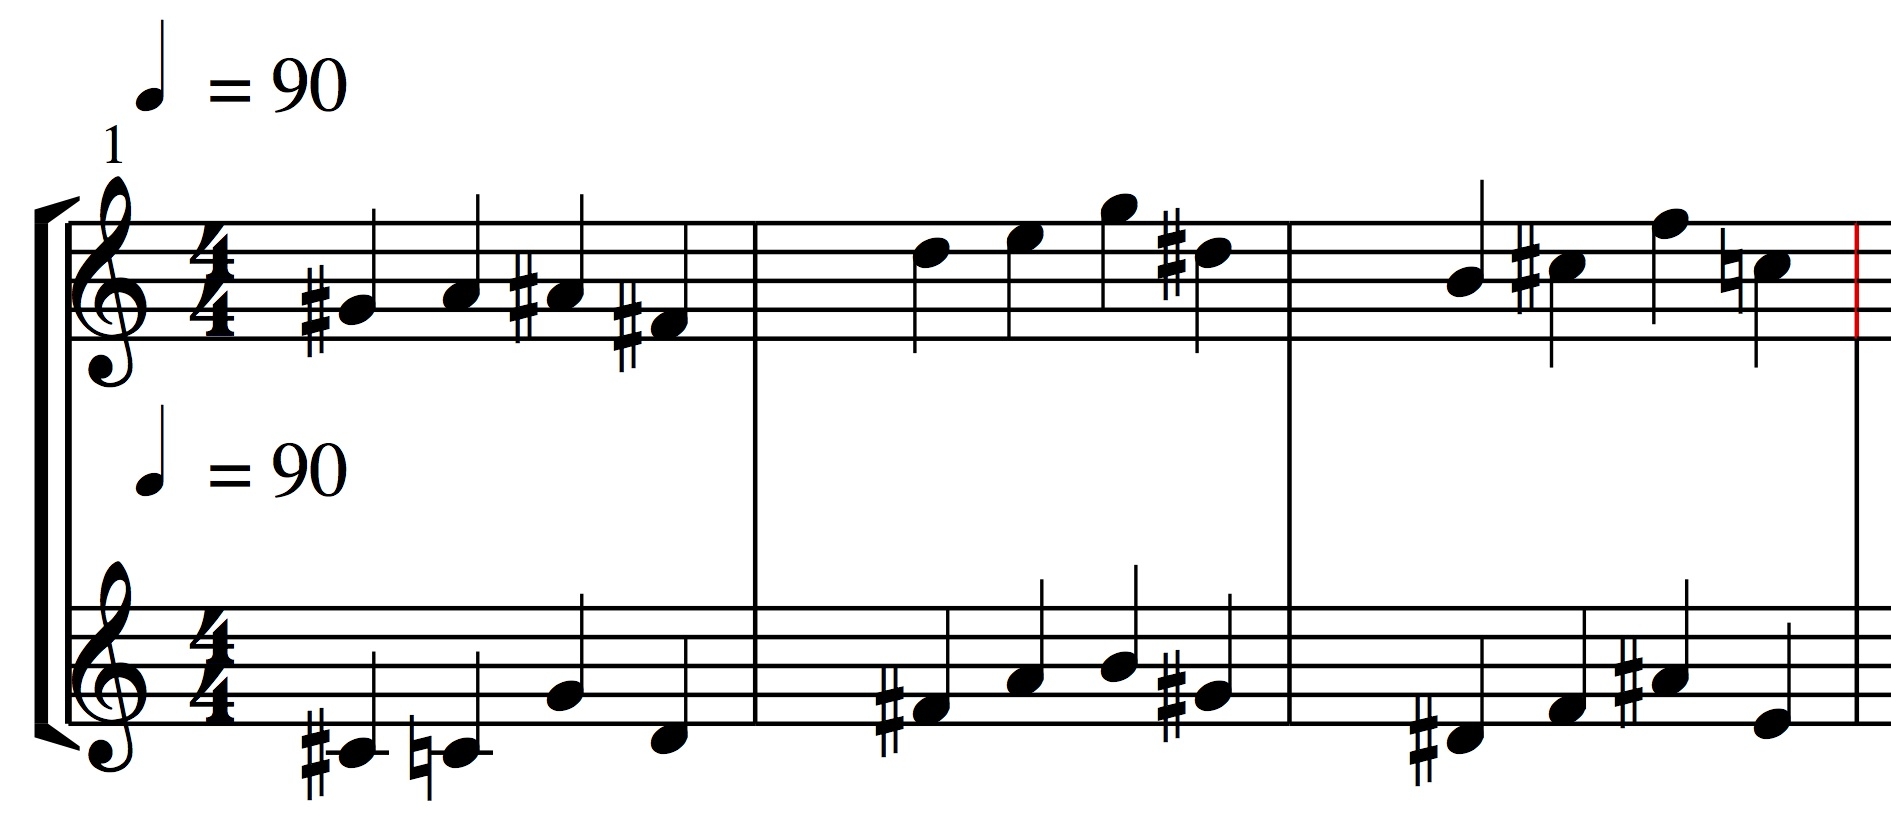
\includegraphics[width=.9\linewidth]{graphics/polyphonic-solution.jpg}
\caption{Possible result of the constraint problem above}
\end{figure}


For further information refer to the PWGL tutorial for now. Pretty much all PWGL boxes have their equivalent Common Lisp function/macro with the same arguments. An exception is the function \texttt{clusterengine} itself, where domains of rhythmic values and pitches are defined in Common Lisp as shown above. 


\subsection*{Cluster Rules}
\label{sec:orgbeb68cb}

The Common Lisp library \href{https://github.com/tanders/cluster-rules}{Cluster Rules} extends Cluster Engine by a collection of predefined musical constraints and that way makes it more easy to use. The equivalent PWGL library is \href{https://github.com/tanders/pwgl-cluster-rules}{PWGL Cluster Rules}. 






\section*{Test}
\label{sec:org2c3885d}

This is a test link to the documentation of function .
\end{document}

% Created 2017-09-21 Thu 12:09
% Intended LaTeX compiler: pdflatex

\section*{API}
\label{sec:org57022d3}

Extracting docs again :)

\begin{description}
\item[{\emph{function} (\textbf{RULES->CLUSTER} \&REST RULES)}] Use this box to collect all rules before inputting them to the Cluster engine. It is possible to input the output of this box to a second Rules->Cluster box (to help organizing your rules in groups).
\end{description}

\begin{description}
\item[{\emph{function} (\textbf{CLUSTERENGINE} NO-OF-VARIABLES RND? DEBUG? RULES METRIC-DOMAIN LIST-OF-DOMAINS)}] The Cluster Engine - the main function of this library.
\end{description}

Pitch domains cannot exist without at least one duration in the rhythm domain. Domains with only one value will not use up any time in the search process.

See the PWGL tutorials of this library for a detailed discussion of this function.

\begin{description}
\item[{\emph{function} (\textbf{R-RHYTHMS-ONE-VOICE} RULE VOICES INPUT-MODE \&OPTIONAL RULE-TYPE WEIGHT)}] :RULE: is a logic statement in he form of a function. The output of the function has to be either true or false. If there are more than one input to the function, they will receive consecutive durations (or consecutive motifs depending on the input-mode).
\end{description}

:VOICES: is the number for the voice (starting at 0) that the rule affects. It is possible to give a list of several voice numbers: The rule will then be applied to every voice in the list (independant of each other).

:INPUT-MODE: determines what type of variables the rule will receive in its inputs:
\begin{itemize}
\item \texttt{:durations} The rule will receive individual durations, one for each input.
\item \texttt{:dur/time} As above, but the start-time of the duration will be indicated.
Format: '(duration start-time), Ex. '(1/4 9/4)
\item \texttt{:motifs} The rule will receive motifs, one (consecutive) motif for each 
input. A motif is a collection of durations that are grouped in 
a list. Motifs are designed in the domain and cannot be 
redesignedby the engine. Note that a motif may be a single 
duration (a list with one duration-ratio) if it is defined as 
such in the domain.
\item \texttt{:motif/time} As the previous selection, but with the start-time of the first event in the motif added. Format: '(motif start-time)
Ex. '((1/4 -1/8) 9/8)
\item \texttt{:all-durations} All durations in the voice that are assigned at the time the rule is checked are given as a list of duration ratios. The list will thus become longer and longer during the search. The rule can only have ONE input in this mode.
\end{itemize}

\textbf{Optional inputs}

By expanding the box it is possible to use the rule as a heuristic switch rule. A heuristic switch rule is still using a logic statement (that outputs true or false), but the effect of the rule is different: If the rule is true, the weight (given in the <weight> input) is passed to the engine. If it is false, a weight of 0 will be passed. A candidate that receive a high weight will have a higher priority for being picked when the true/false rules are checked. A heuristic rule can never fail a candidate, nor can it trigger backtracking of the engine. Heuristic rules only sort the candidates locally before the strict rules are applied. Depending on the context, heuristic rules might have more or less of an effect. 

Heuristic switch rules differs slightly form regular heuristic rules (the latter don't output true or false, but a weight that might vary dependingon the candidate).

[Backtracking: This rule will trigger backtracking in its own engine.]


Here goes on the general text. Here goes on the general text. Here
goes on the general text. Here goes on the general text.



\end{document}


